\documentclass[12pt, a4paper]{article} 
\usepackage{etex}
\usepackage{fontspec}
\usepackage{polyglossia}
\setdefaultlanguage{russian}
\setotherlanguage{english}
\newfontfamily\cyrillicfont{Arial}

\usepackage{hyperref}
\usepackage{amsmath,amsfonts,amssymb,amsthm,mathtools}  

\usepackage{graphicx}
\usepackage{tikzsymbols}
\usepackage{unicode-math}     % пакет для установки математического шрифта
\setmathfont{Asana-Math.otf} 
\renewcommand{\section}{\Smiley{ }}
\renewcommand{\caption}{\Smiley{ }}
\usepackage{graphicx}                  % Для вставки рисунков
\usepackage{graphics} 
\graphicspath{{images/}{pictures/}}    % можно указать папки с картинками
\usepackage{wrapfig}                   % Обтекание рисунков и таблиц текстом
\usepackage{subfigure} 
\usepackage{caption}
\usepackage{tabularx}            % новые типы колонок
\usepackage{tabulary}            % и ещё новые типы колонок
\usepackage{array}               % Дополнительная работа с таблицами
\usepackage{longtable}           % Длинные таблицы
\usepackage{multirow}            % Слияние строк в таблице
\usepackage{float}               % возможность позиционировать объекты в нужном месте 
\usepackage{booktabs}            % таблицы как в книгах!  
\renewcommand{\arraystretch}{1.3} % больше расстояние между строками

\title{Задание 1}
\author{Алиса Жильцова}


\begin{document}

\maketitle

\section{Задание 1. Версия 1}


\begin{figure}[H]
\begin{minipage}[H]{0.32\linewidth} 
 \center 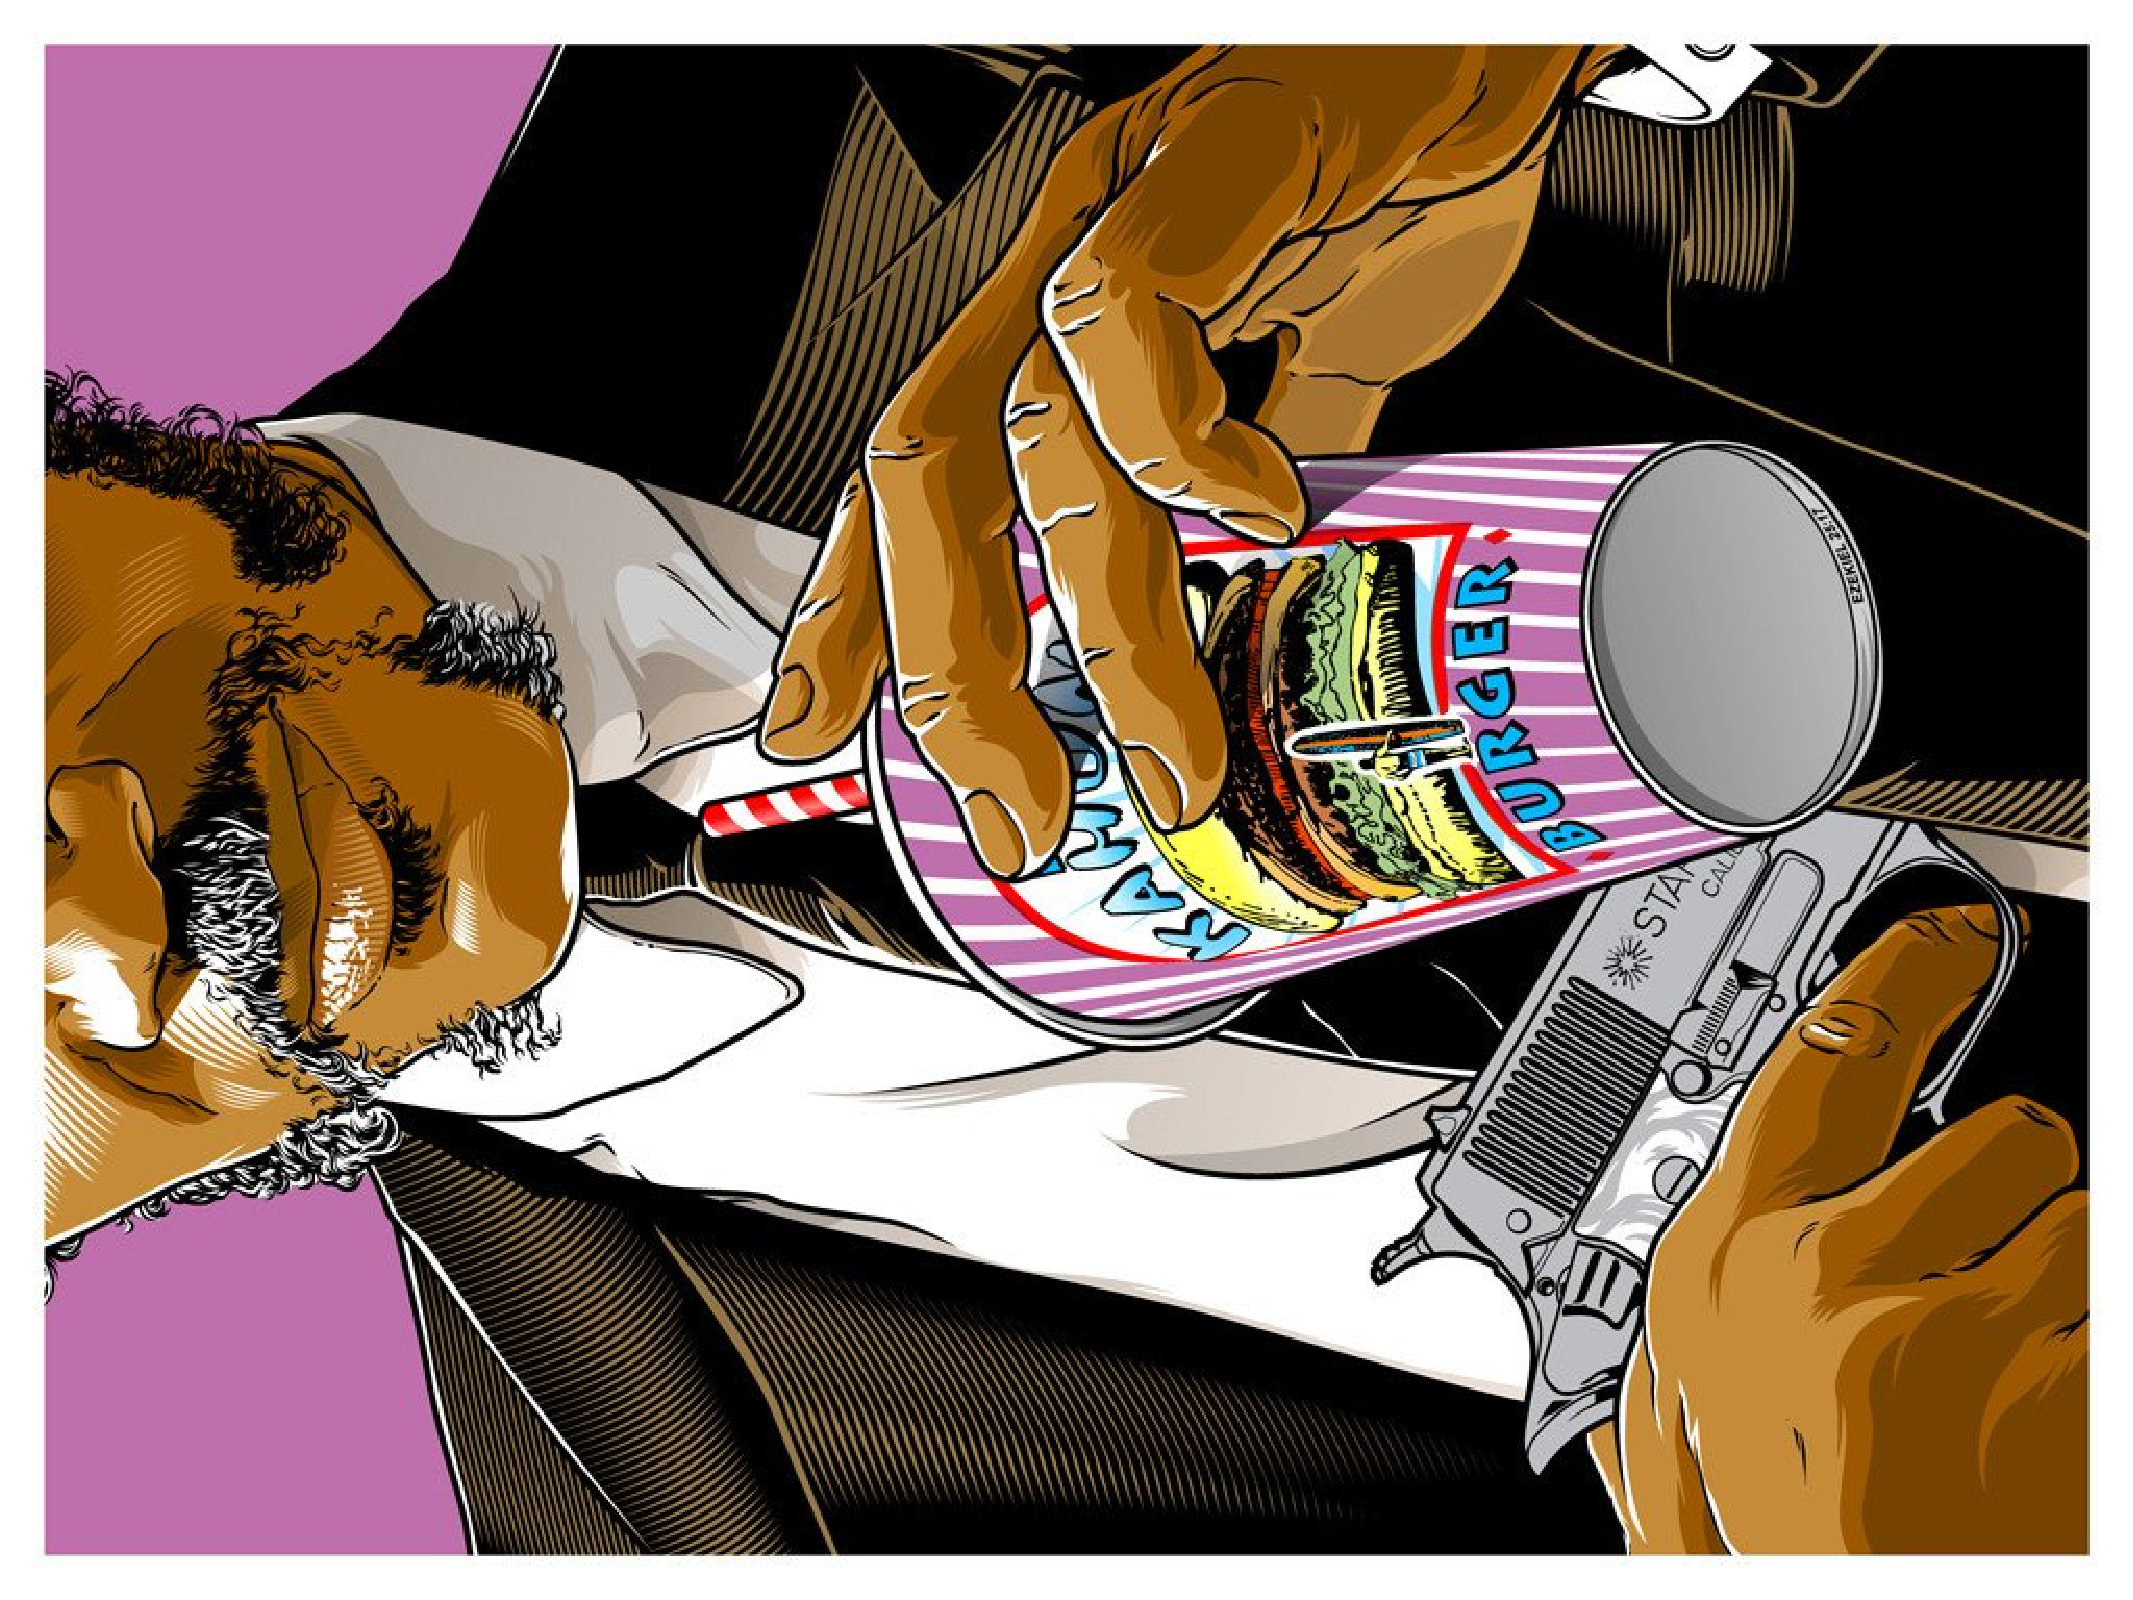
\includegraphics[angle = 270, width= 3.2 cm]{pop1.pdf}
\end{minipage}
\hfill
\begin{minipage}[H]{0.32\linewidth} 
 \center 
\includegraphics[width= 3.3 cm]{pop3.pdf}
\end{minipage}
\hfill
\begin{minipage}[H]{0.32\linewidth} 
 \center 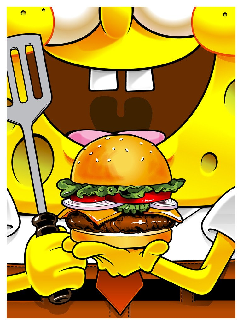
\includegraphics[width= 3.2 cm]{pop8.pdf}
\end{minipage}
\vfill
\begin{minipage}[H]{0.32\linewidth} 
\center 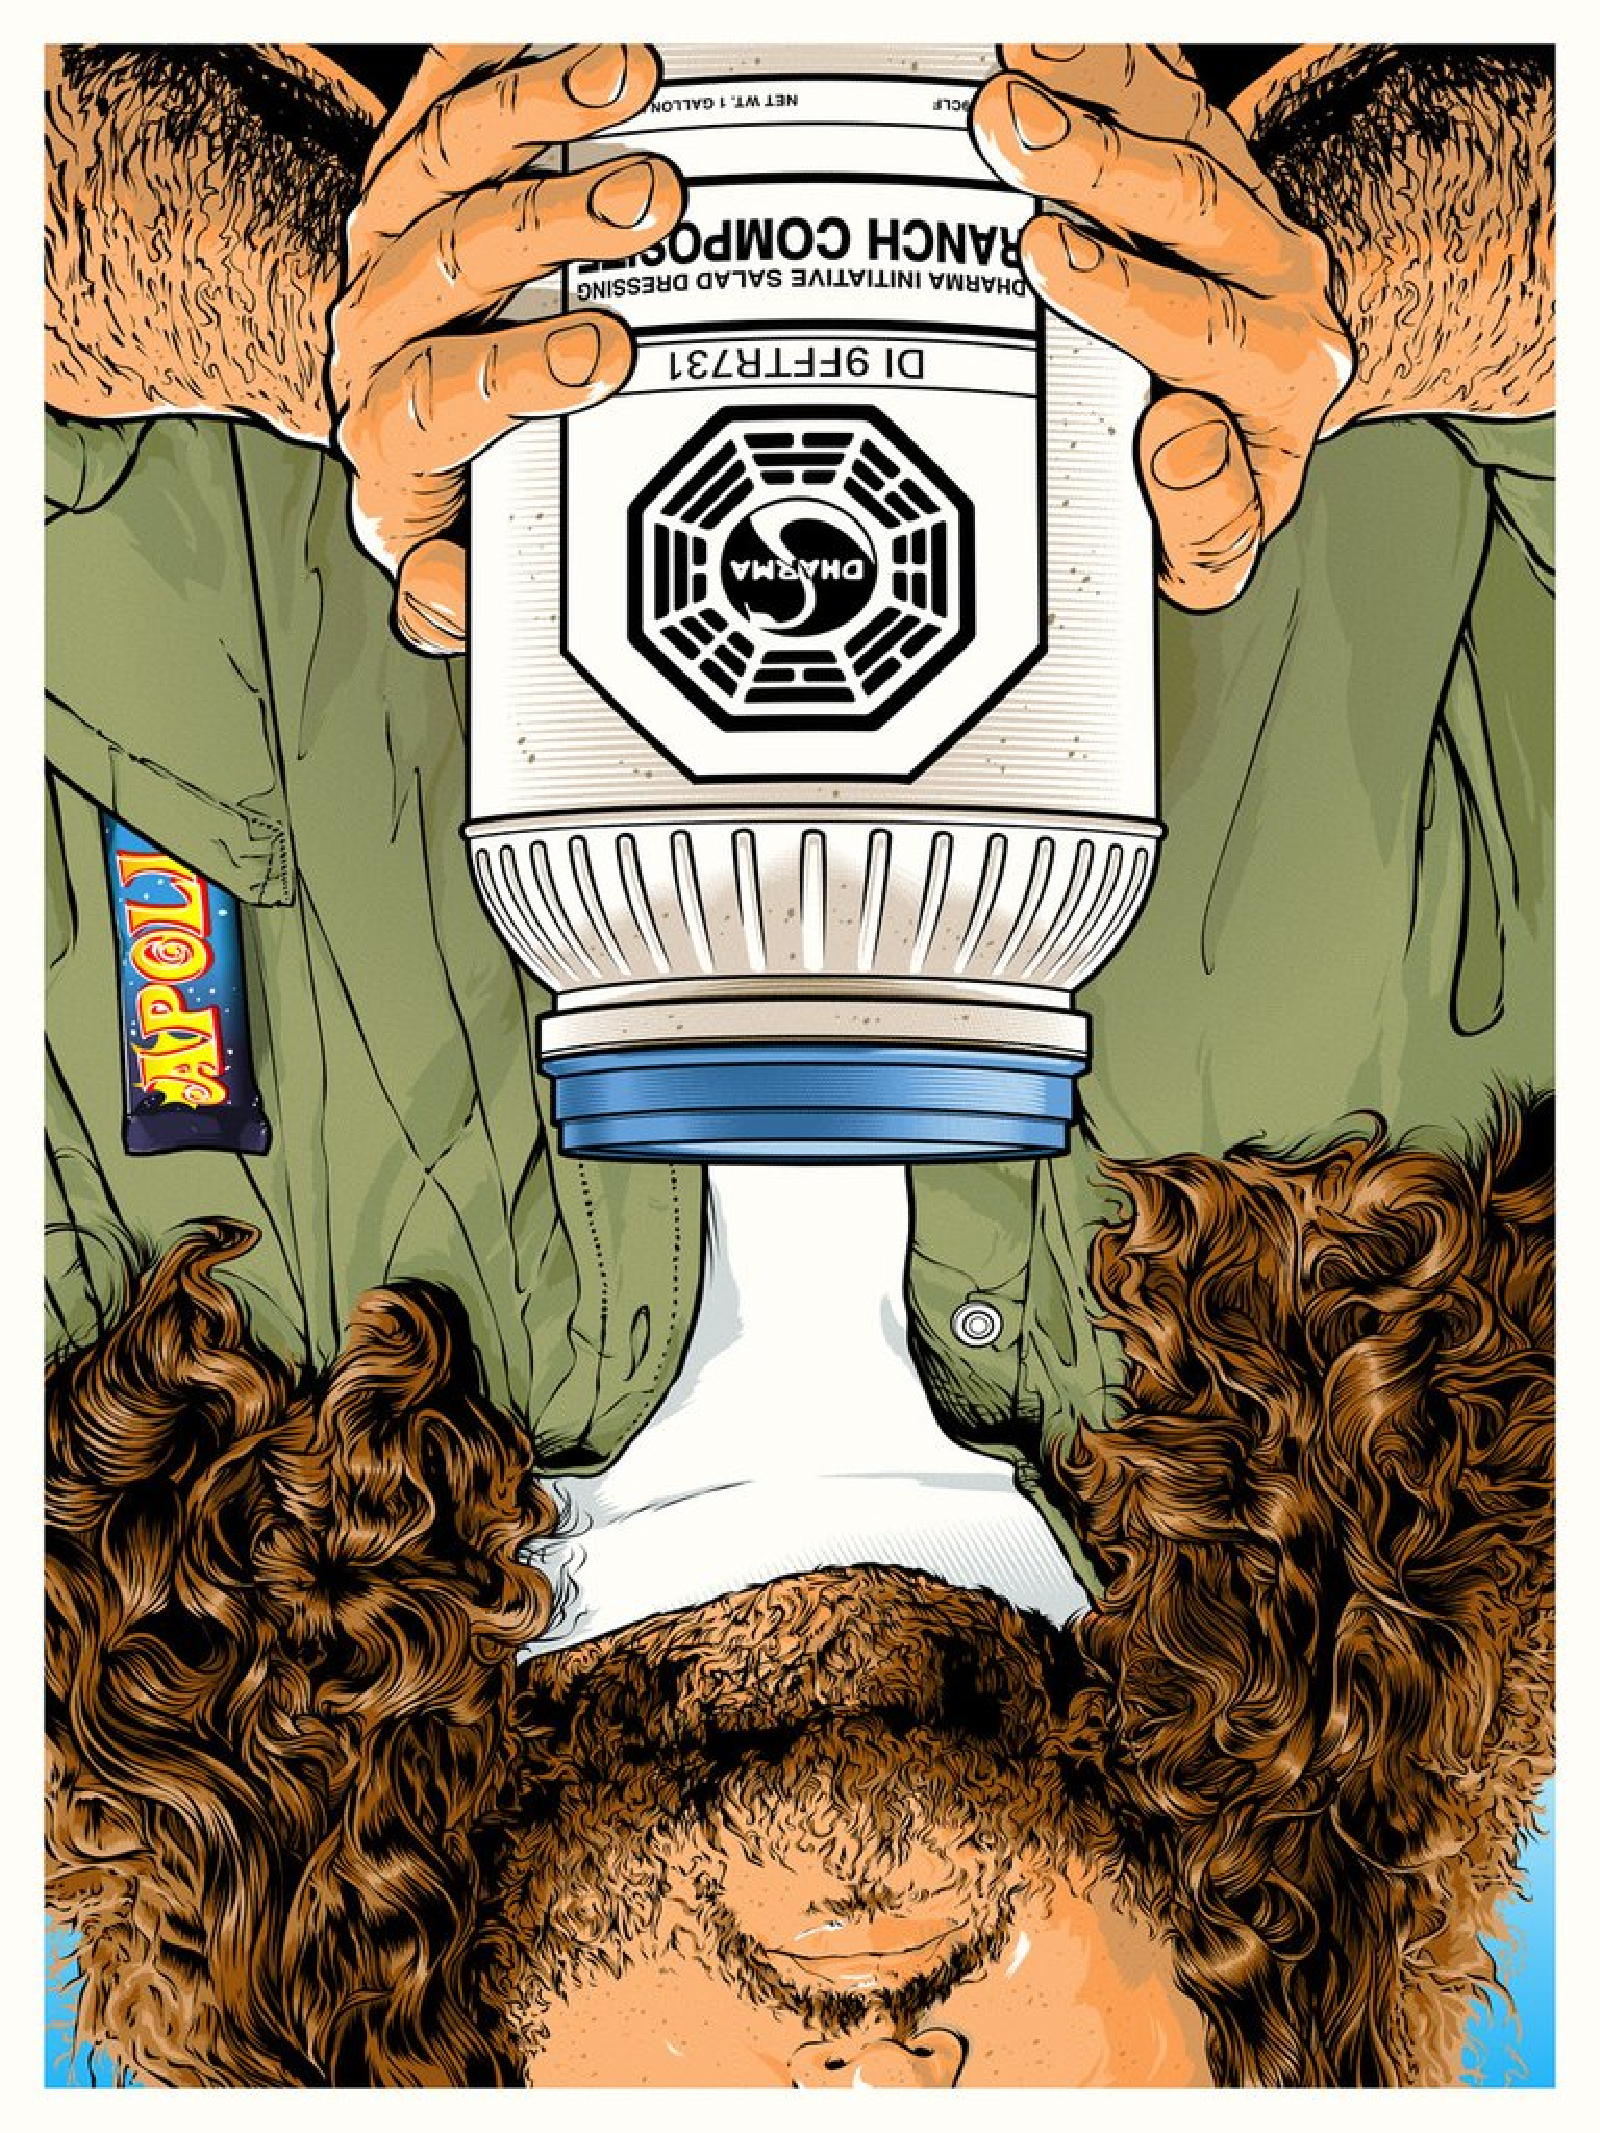
\includegraphics[width= 3.25 cm, angle = 180 ]{pop10.pdf}
\end{minipage}
\hfill
\begin{minipage}[H]{0.32\linewidth} 
\center 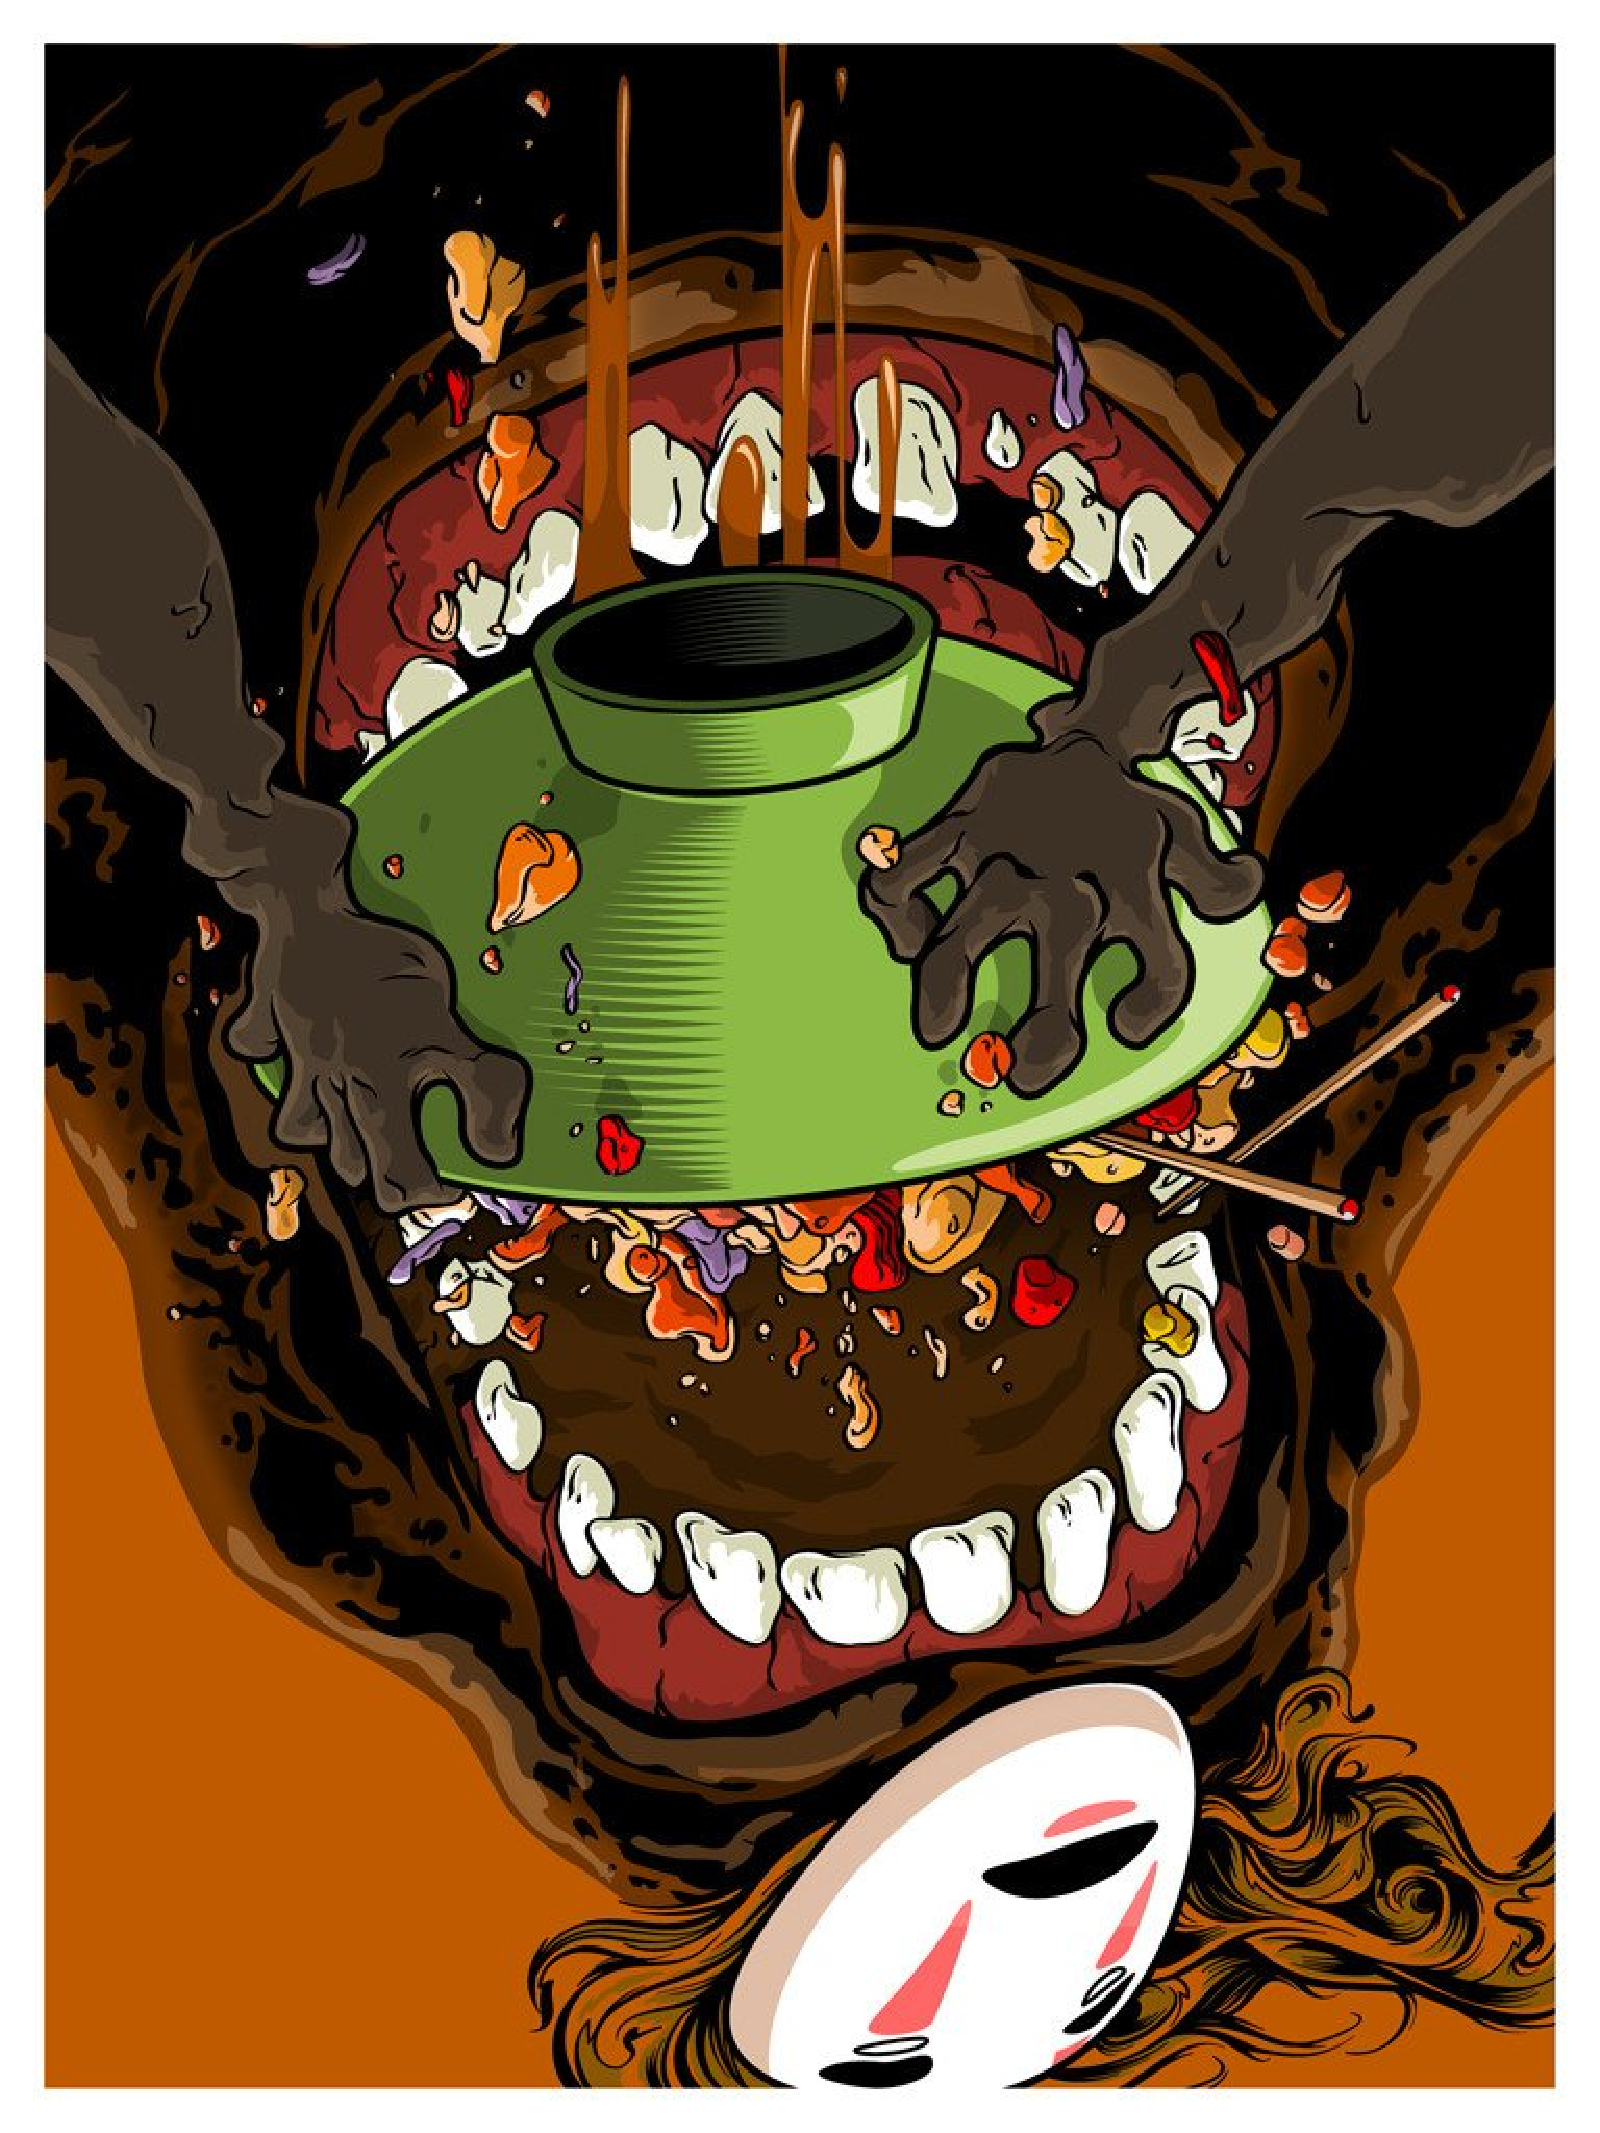
\includegraphics[width= 3.3 cm, angle = 180 ]{pop6.pdf}
\end{minipage}
\hfill
\begin{minipage}[H]{0.32\linewidth} 
\center \includegraphics[width= 3.25 cm ]{pop5.pdf}
\end{minipage}
\caption*{Картинки}
\end{figure}

\newpage

\section{Задание 1. Версия 2}

\begin{table}[H]
\begin{tabular}{m{3.5 cm}m{5 cm}m{3.5  cm}}
 \begin{center} 
\includegraphics[width= 2.1 cm]{pop3.pdf} \end{center}  &  \begin{center} 
\includegraphics[width= 3.5 cm, angle=45]{pop4.pdf} \end{center} &  \begin{center} \includegraphics[width= 2.1 cm ]{pop5.pdf} \end{center} \\
\begin{center} 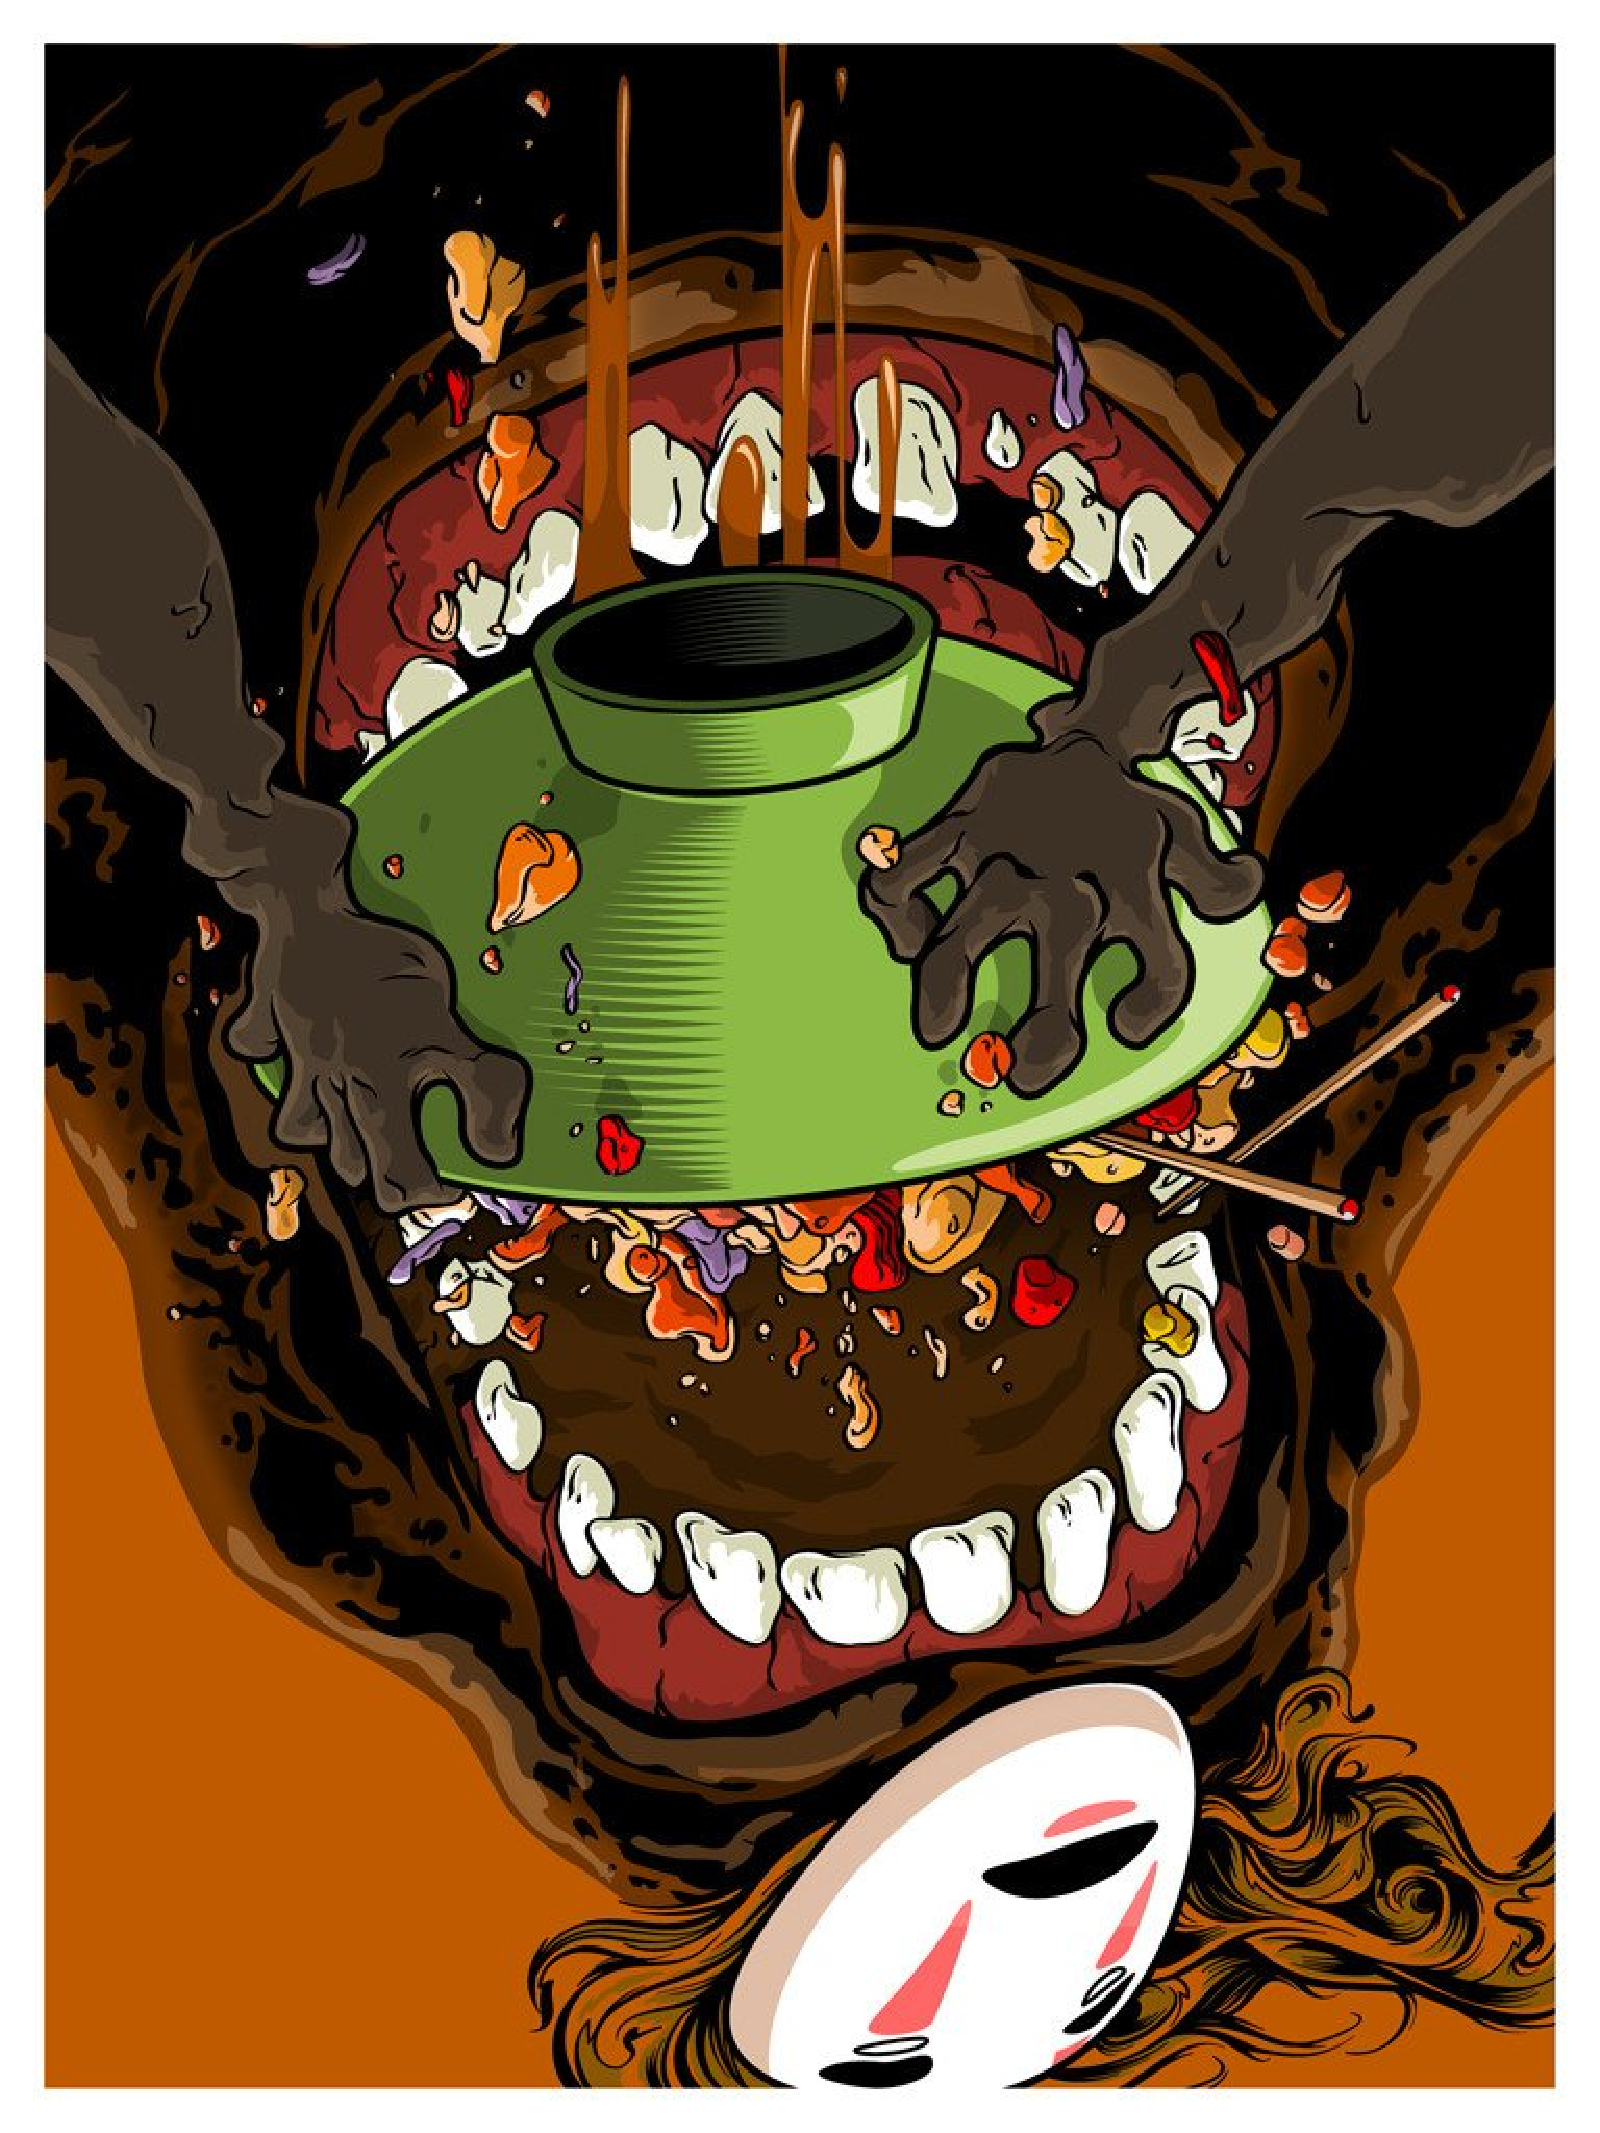
\includegraphics[width= 2.1 cm, angle = 180 ]{pop6.pdf} \end{center} & \begin{center} 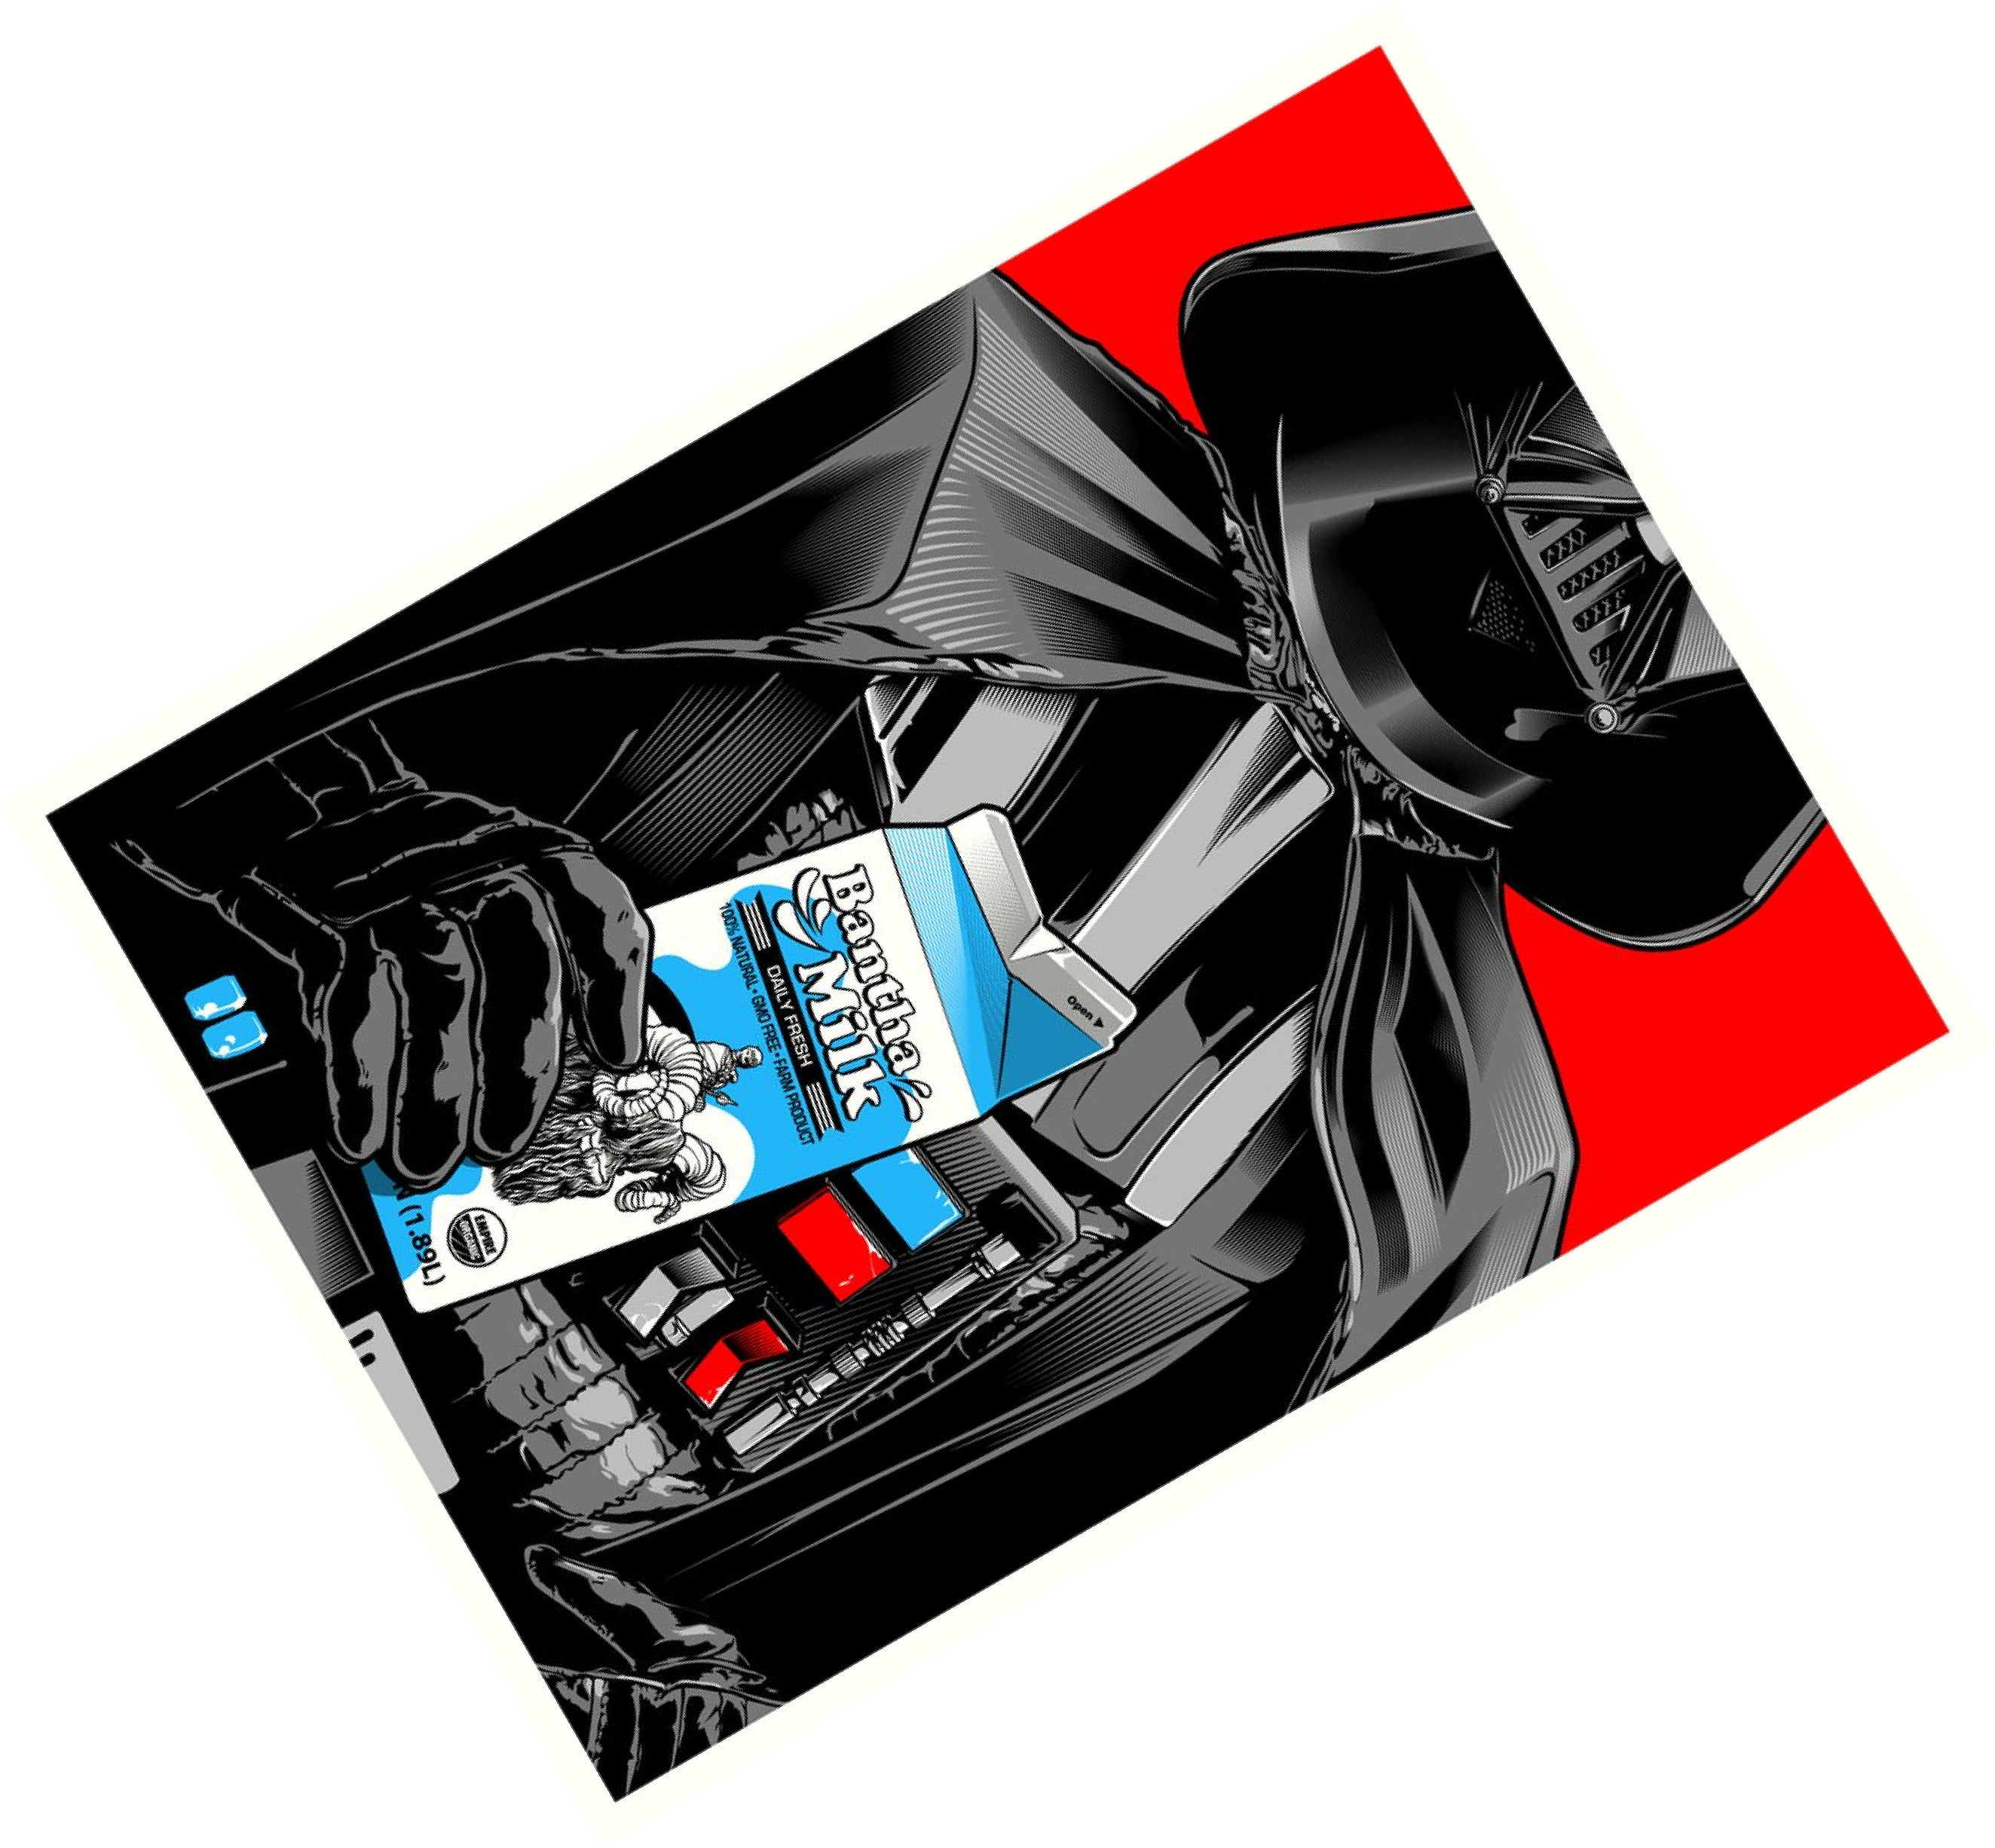
\includegraphics[width= 3.5 cm, angle = 60]{pop9.pdf} \end{center} & \begin{center} 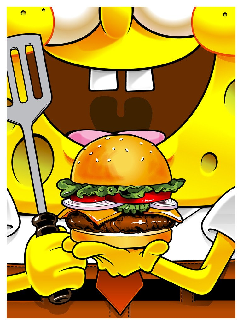
\includegraphics[width= 2.1 cm]{pop8.pdf}\end{center} \\
\end{tabular}
\caption*{Ещё картинки}
\end{table}





\end{document}